% !TEX program = xelatex
\documentclass[aspectratio=169]{beamer}
\usepackage{amsmath}
\usepackage{amssymb}
\usepackage{graphicx}
\usepackage{tcolorbox}
\usepackage{booktabs}
\usepackage{colortbl}
\usepackage{xcolor}
\usepackage{tikz}
\usetikzlibrary{angles,quotes}
\usepackage[utf8]{inputenc}

% Custom colors
\definecolor{primary}{RGB}{41, 128, 185}
\definecolor{secondary}{RGB}{52, 152, 219}
\definecolor{accent}{RGB}{231, 76, 60}
\definecolor{lightgray}{RGB}{236, 240, 241}

% Theme customization
\usetheme{Madrid}
\usecolortheme{whale}
\setbeamercolor{structure}{fg=primary}
\setbeamercolor{background canvas}{bg=white}
\setbeamercolor{normal text}{fg=black}

% Title page info
\title{Pre-Calculus 11}
\subtitle{\textbf{6.1 Basics with Absolute Values and Solving Equations with ABS}}
\author{Created by Yi-Chen Lin}
\date{\today}

\begin{document}

% Title Page
\begin{frame}
    \titlepage
    \vfill
    \centering
    \footnotesize
\end{frame}

% What is an Absolute Value?
\begin{frame}{What is an Absolute Value?}
    \begin{tcolorbox}[colback=lightgray,colframe=primary,title=Definition]
        \footnotesize
        The Absolute value notation is defined as the distance of any value from zero.
        \begin{itemize}
            \item The Absolute value of a positive number stays positive
            \item The ABS of a negative number becomes positive
        \end{itemize}
    \end{tcolorbox}
    \vspace{0.5em}
    \begin{columns}[T,onlytextwidth]
        \column{0.6\textwidth}
        \scriptsize
        \textbf{Examples:}
        \begin{enumerate}[label=(\roman*)]
            \item $|-19| = 19$
            \item $|20| = 20$
            \item $|-81| = 81$
            \item $|-32| = 32$
        \end{enumerate}
    \end{columns}
\end{frame}

% Absolute Value Number Line Concept
\begin{frame}{Absolute Value on a Number Line}
    \begin{tcolorbox}[colback=lightgray,colframe=primary,title=Visualizing Absolute Value]
        \footnotesize
        The absolute value notation is defined as the distance of any value from zero.
    \end{tcolorbox}
    \vspace{0.5em}
    \centering
    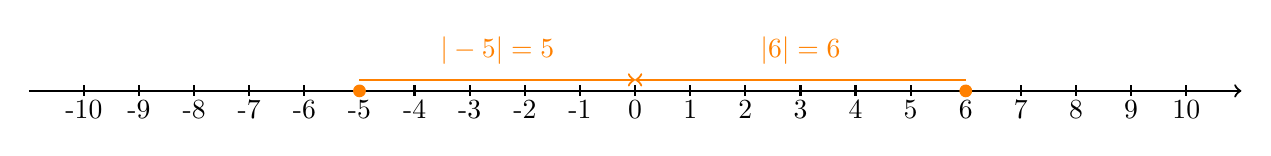
\begin{tikzpicture}[scale=0.7]
        % Draw axis
        \draw[->,thick] (-11,0) -- (11,0);
        % Ticks and labels
        \foreach \x in {-10,-9,...,10} {
            \draw[thick] (\x,0.1) -- (\x,-0.1);
            \ifnum\x>-11 \ifnum\x<11 \node[below] at (\x,0) {\x}; \fi\fi
        }
        % Highlight -5 and 6
        \filldraw[orange] (-5,0) circle (3pt);
        \filldraw[orange] (6,0) circle (3pt);
        % Arrows for distance
        \draw[thick,orange,->] (-5,0.2) -- (0,0.2);
        \draw[thick,orange,->] (6,0.2) -- (0,0.2);
        % Labels
        \node[above,orange] at (-2.5,0.3) {$|-5|=5$};
        \node[above,orange] at (3,0.3) {$|6|=6$};
    \end{tikzpicture}
    \vspace{0.5em}
    \begin{itemize}
        \item The absolute value of a positive number stays positive, but the ABS of a negative number becomes positive.
    \end{itemize}
\end{frame}

% Definition of an Absolute Value
\begin{frame}{Definition of an Absolute Value}
    \begin{tcolorbox}[colback=lightgray,colframe=primary,title=Two Definitions]
        \footnotesize
        \begin{enumerate}
            \item $|x| = \begin{cases} x, & \text{if } x \geq 0 \\ -x, & \text{if } x < 0 \end{cases}$
            \item $|x| = \sqrt{x^2}$
        \end{enumerate}
    \end{tcolorbox}
\end{frame}

% Evaluating ABS Expressions
\begin{frame}{Evaluating ABS Expressions}
    \begin{tcolorbox}[colback=lightgray,colframe=primary,title=Practice]
        \footnotesize
        Evaluate:
        \begin{enumerate}[]
            \item $|25 - 17| = 8$
            \item $|42 - 12| = 30$
            \item $|12 - 317| = 305$
            \item $|432 - 45| = 387$
            \item $|318 - 24| = 294$
        \end{enumerate}
    \end{tcolorbox}
\end{frame}

% Comparing Absolute Values
\begin{frame}{Comparing Absolute Values}
    \begin{tcolorbox}[colback=lightgray,colframe=primary,title=Which is bigger?]
        \footnotesize
        Compare:
        \begin{itemize}
            \item $|132|$ vs $|178|$
            \item $|13|$ vs $|48|$
            \item $|23|$ vs $|-23|$
            \item $|13|$ vs $|-13|$
        \end{itemize}
    \end{tcolorbox}
\end{frame}

% Ordering Numbers
\begin{frame}{Ordering Numbers}
    \begin{tcolorbox}[colback=lightgray,colframe=primary,title=Example 2]
        \footnotesize
        Order from least to greatest:
        \begin{enumerate}[]
            \item $|-7.5|, |-8.2|, |-3.4|, |-14.6|, |-4.3|, |-6.7|, |-12.9|$
            \item $|-5.6|, |-2.1|, |-13.4|, |-24.5|, |-12.3|, |-36.8|, |-25.9|$
        \end{enumerate}
    \end{tcolorbox}
\end{frame}

% Solving Equations with ABS Value
\begin{frame}{Solving Equations with ABS Value}
    \begin{tcolorbox}[colback=lightgray,colframe=primary,title=Key Points]
        \footnotesize
        \begin{itemize}
            \item For $|x| = 10$, $x$ can be $10$ or $-10$
            \item For $|x-5| = 3$, $x-5$ can be $3$ or $-3$
            \item Always check for extraneous roots
        \end{itemize}
    \end{tcolorbox}
\end{frame}

% Practice Problems
\begin{frame}{Practice Problems}
    \begin{tcolorbox}[colback=lightgray,colframe=primary,title=Solve for $x$]
        \footnotesize
        Solve for $x$, indicate if there are any extraneous roots:
        \begin{enumerate}
            \item $|x+5| = 12$
            \item $|2x-4| = 9$
            \item $|3x-7| = 4$
            \item $|x^2-9| = 9$
            \item $|2x^2-12| = 4$
        \end{enumerate}
    \end{tcolorbox}
\end{frame}

% Multiple Choice Questions
\begin{frame}{Multiple Choice Questions}
    \begin{tcolorbox}[colback=lightgray,colframe=primary,title=Practice Questions]
        \footnotesize
        \begin{enumerate}
            \item If $|x+3| = 12$, what are the possible value(s) of $x$?
            \begin{enumerate}[]
                \item $x = 9$
                \item $x = -9$
                \item $x = 15$
                \item $x = -15$
                \item $x = -15$ or $x = 9$
                \item $x = -9$ or $x = 15$
            \end{enumerate}
            
            \item If $|x+5|^2 = 289$, what is the value of $x$?
            \begin{enumerate}[]
                \item $x = 12$
                \item $x = -12$
                \item $x = 22$
                \item $x = -22$
                \item $x = -22$ or $x = 12$
                \item $x = -12$ or $x = 22$
                \item $x = 12$ or $x = 22$
            \end{enumerate}
        \end{enumerate}
    \end{tcolorbox}
\end{frame}

% Challenge Practice Problems

\begin{frame}{Challenge Practice}
    \begin{tcolorbox}[colback=lightgray,colframe=accent,title=Challenge Problems]
        \footnotesize
        \begin{enumerate}
            \item[Q1.] Solve for $x$: $|2x-7| = |x+4|$
            \item[Q2.] Solve for $x$: $|x^2-5x+6| = 2$
        \end{enumerate}
    \end{tcolorbox}
\end{frame}

% Solution to Challenge Q1
\begin{frame}{Challenge Q1 Solution}
    \begin{tcolorbox}[colback=lightgray,colframe=primary,title=Solution to Q1]
        \footnotesize
        $|2x-7| = |x+4|$
        
        \textbf{Case 1:} $2x-7 = x+4$
        \[
        2x-7 = x+4 \\
        2x-x = 4+7 \\
        x = 11
        \]
        \textbf{Case 2:} $2x-7 = -(x+4)$
        \[
        2x-7 = -x-4 \\
        2x+x = -4+7 \\
        3x = 3 \\
        x = 1
        \]
        \textbf{Check for extraneous roots:}
        \begin{itemize}
            \item $x=11$: $|2\times11-7|=|22-7|=|15|=15$, $|11+4|=|15|=15$ (valid)
            \item $x=1$: $|2\times1-7|=|2-7|=|-5|=5$, $|1+4|=|5|=5$ (valid)
        \end{itemize}
        \textbf{Final Answer:} $x=1$ or $x=11$
    \end{tcolorbox}
\end{frame}

% Solution to Challenge Q2
\begin{frame}{Challenge Q2 Solution}
    \begin{tcolorbox}[colback=lightgray,colframe=primary,title=Solution to Q2]
        \footnotesize
        $|x^2-5x+6| = 2$
        
        Let $y = x^2-5x+6$
        
        \textbf{Case 1:} $x^2-5x+6 = 2$
        \[
        x^2-5x+6=2 \\
        x^2-5x+4=0 \\
        (x-4)(x-1)=0 \\
        x=4,\ 1
        \]
        \textbf{Case 2:} $x^2-5x+6 = -2$
        \[
        x^2-5x+6=-2 \\
        x^2-5x+8=0
        \]
        Use quadratic formula:
        \[
        x=\frac{5\pm\sqrt{25-32}}{2}=\frac{5\pm\sqrt{-7}}{2}
        \]
        No real solutions for this case.
        
        \textbf{Final Answer:} $x=1$ or $x=4$
    \end{tcolorbox}
\end{frame}

\end{document} 